\secframe{Thunderbird}{
	Thunderbird\footnote{\url{https://mozilla.org/thunderbird}} ist ein E-Mail Client von Mozilla
	und ist f\"ur die g\"angigen Betriebssysteme verf\"ugbar.
	
	Es gibt weitere E-Mail Clients wie KMail, Evolution, Mutt und so weiter.
}

\subsecframe{Zugriff}{
	Um einen E-Mail Client einzurichten, empfiehlt es sich im Hochschulnetzwerk
	mit seinem Laptop oder im VPN mit seinem Heimrechner zu sein.
	\begin{tip}
    \item Zum Einrichten einer VPN Verbindung siehe die Anleitung des Rechenzentrum\footnote{\url{https://www.htw-dresden.de/rz/vpn}}.
	\end{tip}
}

\subsecframe{Konto einrichten}{
	Zur Einrichtung des E-Mail Kontos ben\"otigt man
	\begin{itemize}
		\item S-Nummer und
		\item Hochschulpassword.
	\end{itemize}
In einigen F\"allen ist es sinnvoll Informationen \"uber den Mail-Server des RZ\footnote{\url{https://www.htw-dresden.de/rz/zentrale-dienste-und-server/e-mail-an-der-htw.html}} zu haben.
	\begin{itemize}
		\item Incoming
	\begin{description}
		\item[Server hostname] imap.htw-dresden.de
		\item[Port] 143
		\item[SSL] STARTTLS
		\item[Authentication] Normal password
	\end{description}
		\item Outgoing
	\begin{description}
		\item[Server hostname] mail.htw-dresden.de
		\item[Port] 25
		\item[SSL] STARTTLS
		\item[Authentication] Normal password
	\end{description}
	\end{itemize}
}

\frame{
    \frametitle{Konto einrichten II}
    \begin{columns}
        \begin{column}{0.5\textwidth}
            \begin{figure}[!h]
                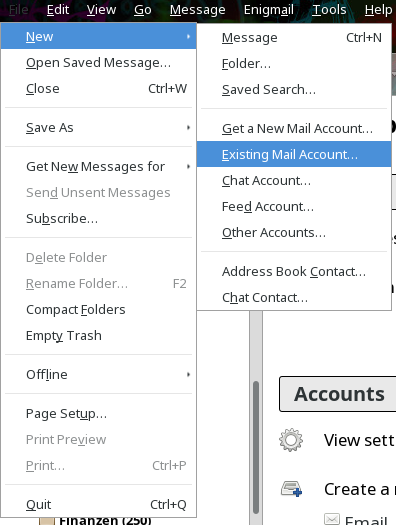
\includegraphics[width=0.7\textwidth]{../images/tb_new_mail_account.png}
            \end{figure}
        \end{column}
        \begin{column}{0.5\textwidth}
            \begin{description}
                \item[1.] File/Datei
                \item[2.] New/Neu
                \item[3.] Exisiting Mail account/ Mail-Konto
            \end{description}
        \end{column}
    \end{columns}
}

\frame{
	\frametitle{Konto einrichten III}
	 \begin{figure}[!h]
		 \centering
		 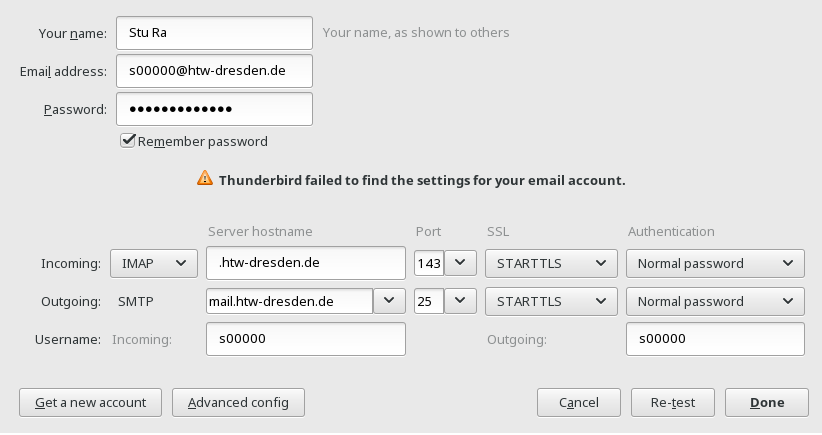
\includegraphics[width=0.9\textwidth]{../images/tb_new_mail_account_II.png}
		 \vspace{-20pt}
	 \end{figure}
 }

\subsecframe{Ordner anlegen}{
	\begin{minipage}[b]{0.35\linewidth}
		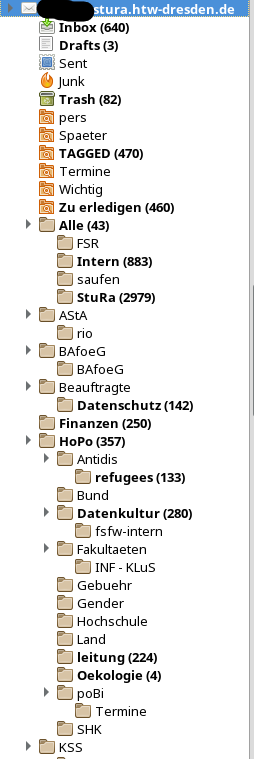
\includegraphics[height=0.8\textheight]{../images/tb_filestruct.png}
	\end{minipage}
	\begin{minipage}[t]{0.63\linewidth}
		\vspace{-5cm}
		\large
	Das Erstellen von Ordnern hilft bei der Klassifizierung und Sortierung der erhaltenen e-Mails.
	\end{minipage}
}

\frame{
	\frametitle{Ordner anlegen II}
	   \begin{figure}
	   \subfigure[Ordner anlegen] {
		   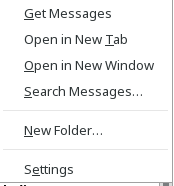
\includegraphics[height=0.5\textheight]{../images/tb_new_folder_I.png}
		   }
	   \subfigure[Unterordner anlegen] {
		   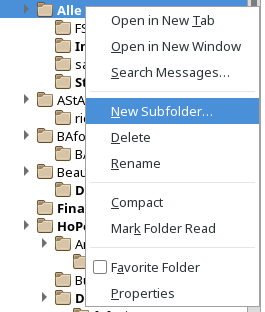
\includegraphics[height=0.5\textheight]{../images/tb_new_subfolder_I.png}
		   }
	   \end{figure}
	   \textit{Rechtsklick} $->$ New Folder oder New Subfolder
   }

\frame{
	\frametitle{Ordner anlegen III}
	   \begin{figure}
		   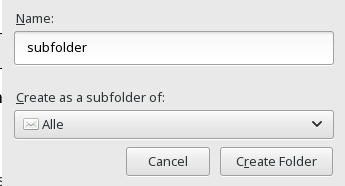
\includegraphics[height=0.5\textheight]{../images/tb_new_subfolder_II.png}
	   \end{figure}
	\begin{description}
		\item[Name:] Name des Ordners
		\item[Create as a subfolder of:] Erstelle als Unterordner von:
	\end{description}
	}

\subsecframe{Manage Identities / Aliases}{
	Accounts $->$ View settings for this account $->$ Manage Identities $->$ Add
	Konten $->$ Zeige Kontoeinstellungen $->$ 
   \begin{figure}
	   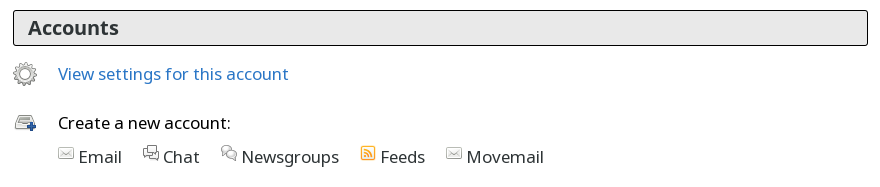
\includegraphics[width=\textwidth]{../images/tb_accounts.png}
   \end{figure}
}

\frame {
    \frametitle{Manage Identities / Aliases II}
    \begin{columns}
        \begin{column}{0.5\textwidth}
            \begin{figure}
                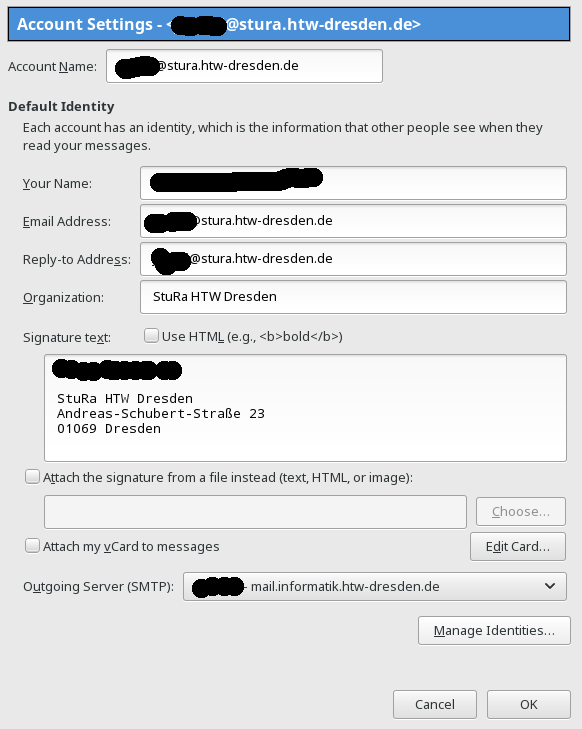
\includegraphics[width=\textwidth]{../images/tb_account_settings.png}
            \end{figure}
        \end{column}
        \begin{column}{0.53\textwidth}  %%<--- here
            \begin{description}
                \item[Account Name:] frei w\"ahlbar
                \item[Your Name:] Vorname Nachname
                \item[Email Address:] nachname@stura.htw-dresden.de
                \item[Replay-To Address:] selbe wie Email Adresse
                \item[Organization:] StuRa HTW Dresden
                \item[Signature text:] Vorname Nachname\newline
                    \newline
                    StuRa HTW Dresden\newline
                    Andreas-Schubert-Str. 23\newline
                    01069 Dresden
                \item[Outgoing Server (SMTP):] mail.htw-dresden.de
            \end{description}
        \end{column}
    \end{columns}
}

\frame {
	\frametitle{Manage Identities / Aliases III}
   \begin{figure}
	   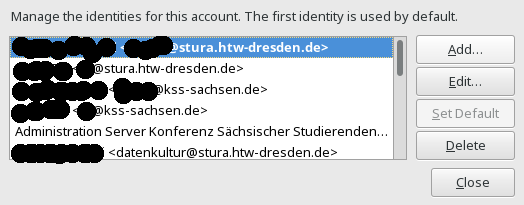
\includegraphics[width=\textwidth]{../images/tb_manage_identities.png}
   \end{figure}
   Es ist praktisch Aliases f\"ur die Bereiche und Referate zuerstellen.
}

\frame {
	\frametitle{Manage Identities / Aliases IV}

    \begin{columns}
        \begin{column}{0.5\textwidth}
            \begin{figure}
                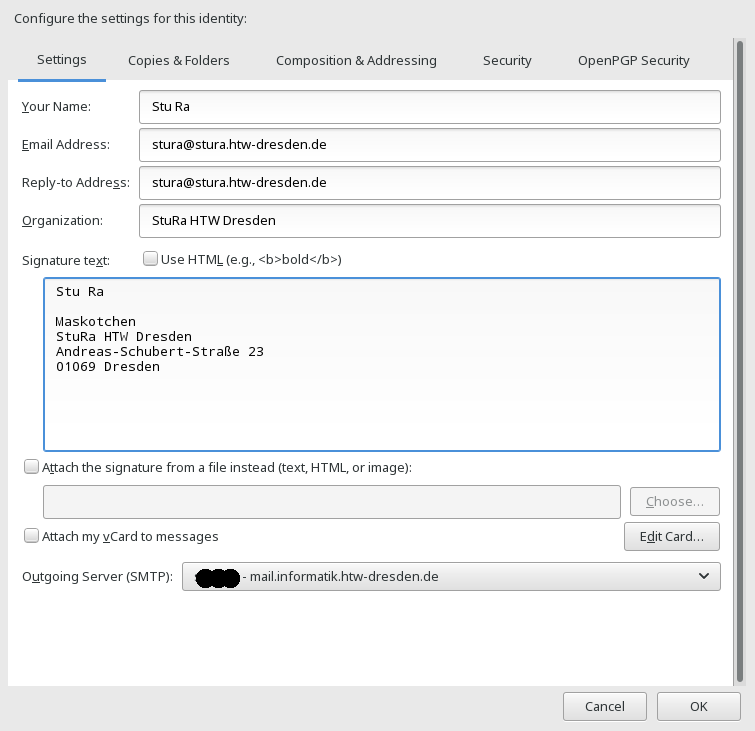
\includegraphics[width=\textwidth]{../images/tb_add_identitie.png}
            \end{figure}
        \end{column}
        \begin{column}{0.53\textwidth}  %%<--- here
            \begin{description}
                \item[Account Name:] frei w\"ahlbar
                \item[Your Name:] Funktion
                \item[Email Address:] funktion@stura.htw-dresden.de
                \item[Replay-To Address:] selbe wie Email Adresse
                \item[Organization:] StuRa HTW Dresden
                \item[Signature text:] Funktion\newline
                    \newline
                    StuRa HTW Dresden\newline
                    Andreas-Schubert-Str. 23\newline
                    01069 Dresden
                \item[Outgoing Server (SMTP):] mail.htw-dresden.de
            \end{description}
        \end{column}
    \end{columns}
}

\subsecframe{Filter} {
   \begin{figure}
	   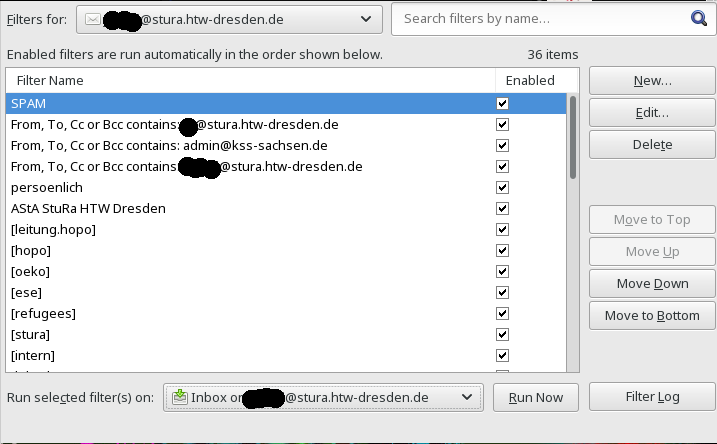
\includegraphics[height=0.8\textheight]{../images/tb_message_filters.png}
   \end{figure}
	
}

\frame {
	\frametitle{Filter II}
   \begin{figure}
	   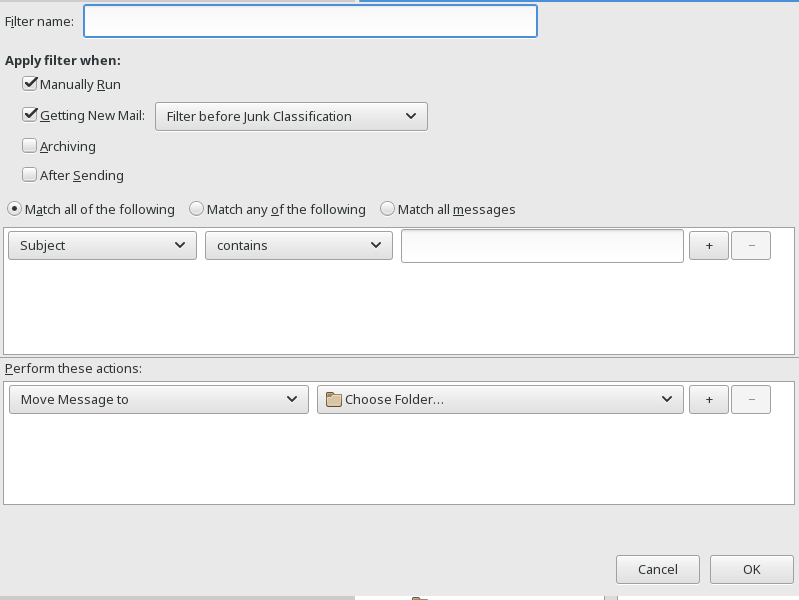
\includegraphics[height=0.8\textheight]{../images/tb_new_filter_rules.png}
   \end{figure}

}
\frame{
	\frametitle{Spamfilter}
   \begin{figure}
	   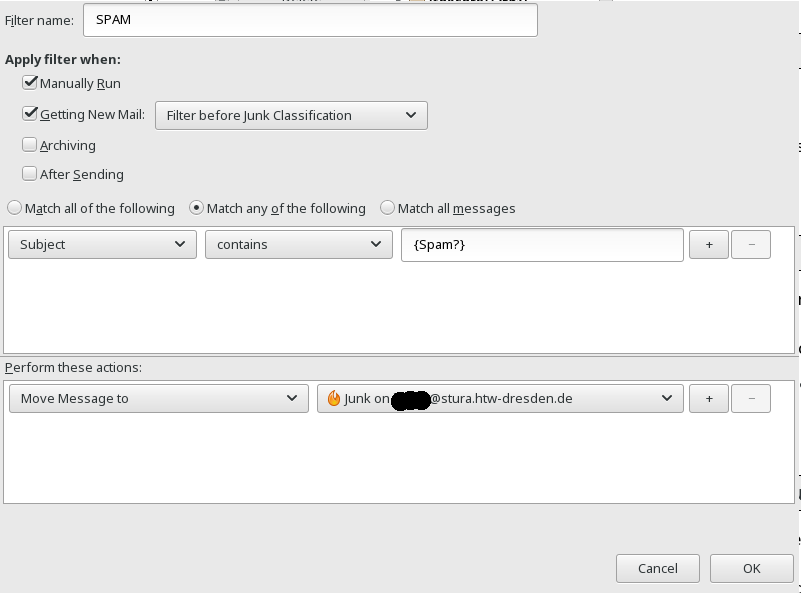
\includegraphics[height=0.8\textheight]{../images/tb_new_spam_filter_rule.png}
   \end{figure}
}
%%%spamfilter
%%%sortieren
